\problem{}
\subproblem{}
از لحاظ مفهومی چولگی به معنای میزان دوری داده های پرت است یا به عبارتی علامت آن نشان دهنده راست یا چپ بودن داده های دور تر از میانگین یا مد است.

\subproblem{}
\begin{figure}[H]
	\centering
	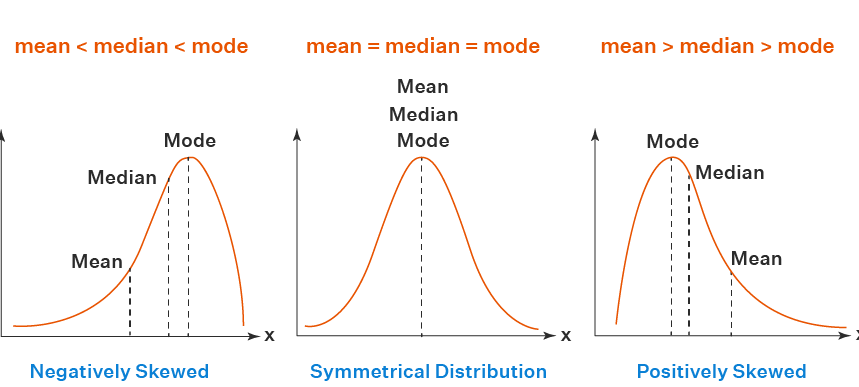
\includegraphics[width=0.5\textwidth]{/Users/kajal/Documents/statistics/resources/hw1/skewness.png}
\end{figure}
شکل بالا به وضوح به ما نشان میدهد که ترتیب میانگین و میانه و مد در چولگی به چپ و راست و توزیع متقارن به چه صورت است.
\\
\subproblem{}
برابر بودن ضریب اول و دوم پیرسن به ما رابطه زیر را می دهند:
\[
\frac{\bar{x} - M}{s} = \frac{3(\bar{x} - m)}{s} = 0.32
\]
که با قرار دادن میانگین و انحراف معیار به ترتیب داریم:
\[
\frac{29.6 - M}{6.5} = 0.32
\]
که به ما می‌دهد:
\[ M = 29.6 - (0.32 \times 6.5) = 27.52 \text{ (مد)} \]
و برای معادله دوم:
\[
\frac{3(29.6 - m)}{6.5} = 0.32
\]
که به ما می‌دهد:
\[ 29.6 - m = 0.693 \]
بنابراین:
\[ m \approx 29.6 - 0.693 = 28.907 \approx 28.9 \]
